\chapter{リアルタイム看板認識APIの実装}
\label{chapter:implement_recog}
本章では,リアルタイムで看板認識を行うために実装したAPIについて述べる.

\section{システムの概要}
  リアルタイムでカメラを通して見た映像に店舗情報を付与するために,街を撮影した画像から看板を認識し,その結果をJSON形式で返却するAPIを実装した\cite{Kitamura:2018}.
  APIは看板を2段階で認識する.
  まず,APIはYOLOv2 \cite{Redmon:2017}を用いて画像の中から看板を囲む長方形の枠線であるバウンディングボックスを検出する.
  次に,YOLOによって切り出された看板をVGG16 \cite{Simonyan:2015}を用いて店舗毎にクラス分けを行う.
  これにより,少ない教師データから高精度での看板認識が可能になる.
  
\section{対象とするデータ}
  本稿では,大阪府高槻市のJR高槻駅と阪急高槻市駅の間に位置する商店街の一区域を対象としたプロトタイプを実装する.
  プロトタイプでは,図\ref{figure:recog_map}の赤線部で示されている高槻本通の$100\, \mathrm{m}$区間において,オープンソースの地理情報システムであるOpenStreetMap(以下,OSMと記す)\cite{Haklay:2008}に2018年10月1日時点でデータが存在した15店舗(赤から 高槻店,メサベルテ 高槻店,高槻ちゃぶちゃぶ,炭焼酒場 森田屋 高槻店,全席個室居酒屋 北海の恩返し 高槻店,肉丼専門店 高槻肉劇場,磯丸水産 高槻店,おだいどこはなれ 高槻店,ぢどり亭 高槻店,ビリヤード・ダーツ \& Food Bar OzBuddy,小だるま JR高槻駅前店,焼肉・しゃぶしゃぶ食べ放題 ぷくぷく 高槻店,甲南チケット 高槻本通店,セブン--イレブン 高槻高槻町店,駿河屋)を対象とする.
  \begin{figure}[tb]
    \centerline{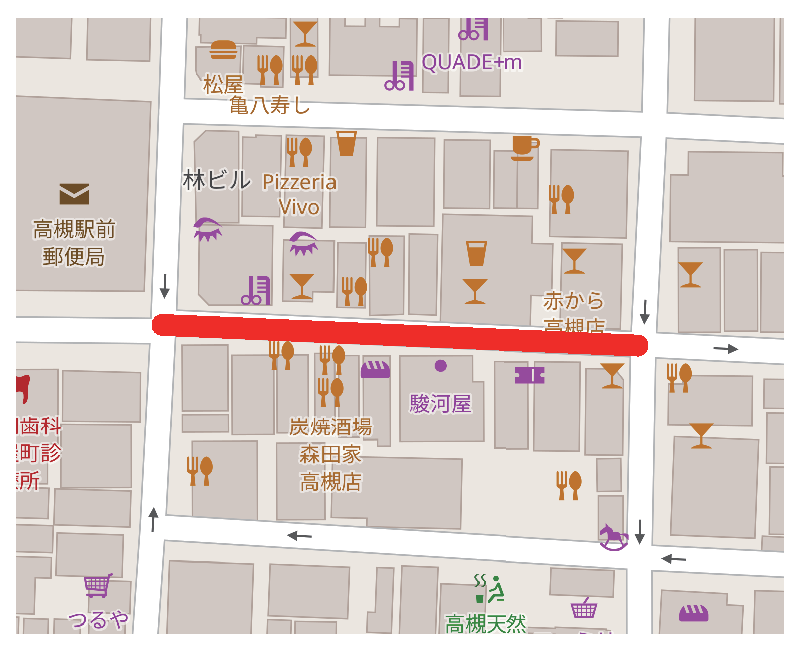
\includegraphics[width=\columnwidth, clip]{recog_map.eps}}
    \caption{対象とする区域}
    \label{figure:recog_map}
  \end{figure}

\section{看板領域の抽出}

\section{抽出した看板の分類}

  In order to confirm that signboards can be recognized instantly, % in the real world,
  %現実世界でその場で看板を認識できることを確かめるために,
  we collected 650 images from around 15 stores in one area of the shopping street of Takatsuki city, Osaka prefecture,
  and annotated the signboard area in those images.
  %大阪府高槻市の商店街の1区画にある15店舗の周辺で650枚の写真を収集し,看板の領域をアノテーションした.
  Then, we used 585 pictures as training data and 65 pictures as test data using YOLO.
  %585枚の写真を教師データ,65枚の写真をテストデータとしてYOLOに学習させた.
  In addition, we collected 100 signboard pictures from 15 stores in the area.
  %さらに,15店舗の看板画像を100枚ずつ収集した.
  For each store, we selected 50 pictures for training data, 25 pictures for validation data,  and 25 pictures for test data. Training was performed using VGG16.
  %1店舗につき教師データ50枚,バリデーションデータ25枚,テストデータ25枚に分け,VGG16に学習させた.
  The accuracy of signboard recognition using test data was 95\%.
  %テストデータでの精度は95%であった.
  %We implemented an Android application that can call the API.
  Subsequently, verification was performed using field experiments.
  %APIを呼べるAndroidアプリを実装し,実地で精度に関する実験を行った.

\section{精度に関する実験}
  In the experiment, we sent images of the front of the store to the API ten times and counted the number of times that (a) the signboard area was detected correctly; and (b) the signboard images were properly classified.
  %実験では,各店舗の前で10回ずつAPIに画像を送信し,(a)看板領域が正しく検出された回数,(b)看板画像が正しくクラス分けされた回数,を測定した.
  The results of the experiment are shown in Table \ref{table:recog_result}.
  %実験結果を表1に示す.
  The overall recognition accuracy was 86\%, and recognition was performed within 1 second.
  Recognition in real-time was achieved by calling the API every 500 milliseconds.
  %全体の認識精度は86%であり,500ms毎にAPIを呼び出せばリアルタイムでの認識も可能だった.
  In the event that the same store had a number of similar signboards, then the recognition accuracy appeared to decrease.
  %同一店舗に類似していない複数枚の看板がある場合,認識の精度が低くなる傾向が見られた.
  This framework allows users to intuitively access store information from signboards.
  %このフレームワークはユーザが看板から店舗の情報に直感的にアクセスすることを可能にする.

  \begin{table}[t]
    \caption{実験の結果}
    \label{table:recog_result}
    \begin{center}
      \begin{tabular}{cc|cc}
        \hline\hline
        店舗名 & 看板画像 & (a) & (b) \\ \hline
        %1
        赤から 高槻店 & 
        \begin{minipage}{40mm}
          \centering
          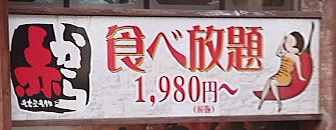
\includegraphics[clip, height=2zh]{akakara.jpg}
        \end{minipage} & 9 & 9 \\
        メサベルテ 高槻店 & 
        \begin{minipage}{40mm}
          \centering
          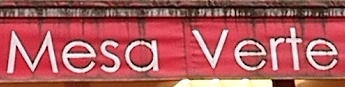
\includegraphics[clip, height=2zh]{mesaverte.jpg}
        \end{minipage} & 10 & 10 \\
        %2
        高槻ちゃぶちゃぶ & 
        \begin{minipage}{40mm}
          \centering
          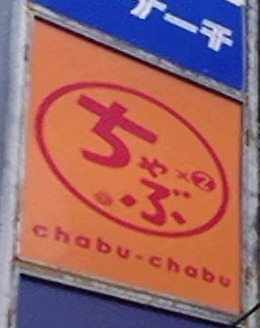
\includegraphics[clip, height=2zh]{chabuchabu.jpg}
        \end{minipage} & 9 & 9 \\
        炭焼酒場 森田屋 高槻店 & 
        \begin{minipage}{40mm}
          \centering
          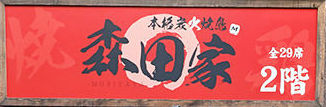
\includegraphics[clip, height=2zh]{moritaya.jpg}
        \end{minipage} & 10 & 10 \\
        %3
        全席個室居酒屋 北海の恩返し 高槻店 & 
        \begin{minipage}{40mm}
          \centering
          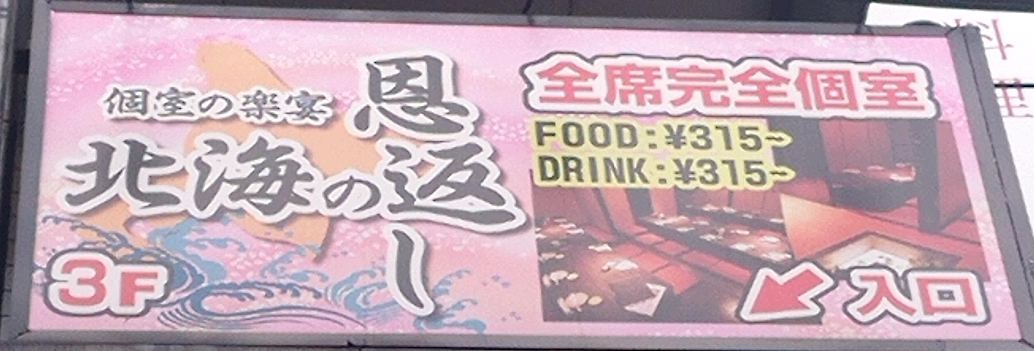
\includegraphics[clip, height=2zh]{hokkai.jpg}
        \end{minipage} & 10 & 10 \\
        肉丼専門店 高槻肉劇場 & 
        \begin{minipage}{40mm}
          \centering
          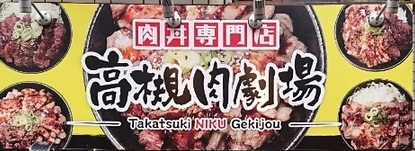
\includegraphics[clip, height=2zh]{nikugekijo.jpg}
        \end{minipage} & 9 & 9 \\
        %4
        磯丸水産 高槻店 & 
        \begin{minipage}{40mm}
          \centering
          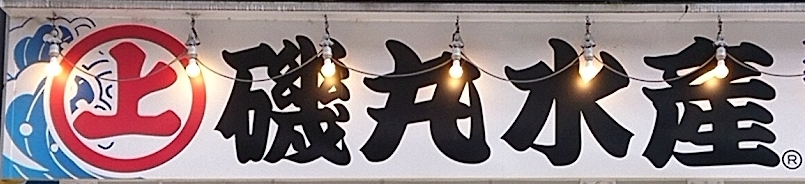
\includegraphics[clip, height=2zh]{isomaru.jpg}
        \end{minipage} & 10 & 10 \\
        おだいどこはなれ 高槻店 & 
        \begin{minipage}{40mm}
          \centering
          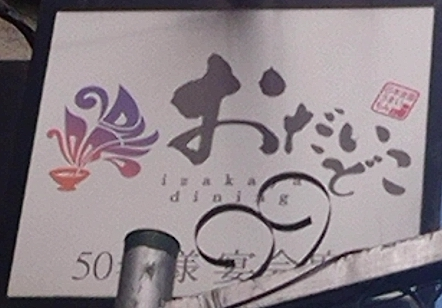
\includegraphics[clip, height=2zh]{odaidoko.jpg}
        \end{minipage} & 8 & 3 \\
        %5
        ぢどり亭 高槻店 & 
        \begin{minipage}{40mm}
          \centering
          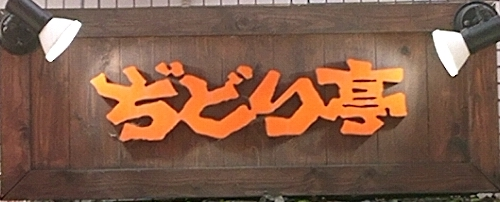
\includegraphics[clip, height=2zh]{jidori.jpg}
        \end{minipage} & 10 & 7 \\
        ビリヤード・ダーツ \& Food Bar OzBuddy & 
        \begin{minipage}{40mm}
          \centering
          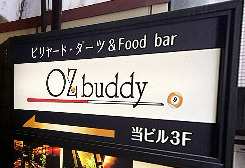
\includegraphics[clip, height=2zh]{ozbuddy.jpg}
        \end{minipage} & 10 & 10 \\
        %6
        小だるま JR高槻駅前店 &
        \begin{minipage}{40mm}
          \centering
          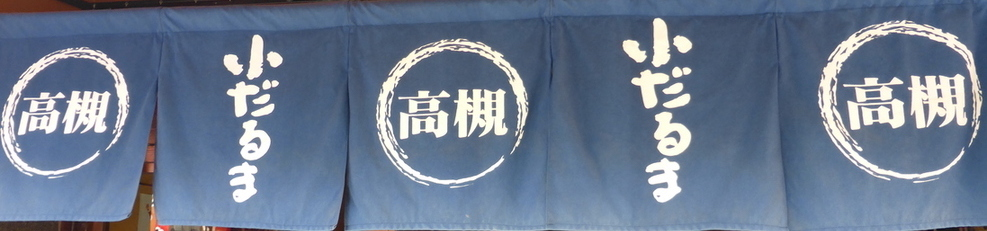
\includegraphics[clip, height=2zh]{kodaruma.jpg}
        \end{minipage} & 10 & 10 \\
        焼肉・しゃぶしゃぶ食べ放題 ぷくぷく 高槻店 & 
        \begin{minipage}{40mm}
          \centering
          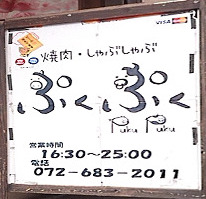
\includegraphics[clip, height=2zh]{pukupuku.jpg}
        \end{minipage} & 10 & 10 \\
        %7
        甲南チケット 高槻本通店 & 
        \begin{minipage}{40mm}
          \centering
          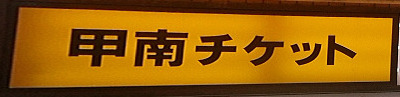
\includegraphics[clip, height=2zh]{konan.jpg}
        \end{minipage} & 8 & 8 \\
        セブン--イレブン 高槻高槻町店 & 
        \begin{minipage}{40mm}
          \centering
          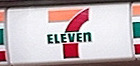
\includegraphics[clip, height=2zh]{seveneleven.jpg}
        \end{minipage} & 9 & 9 \\
        %8
        駿河屋 & 
        \begin{minipage}{40mm}
          \centering
          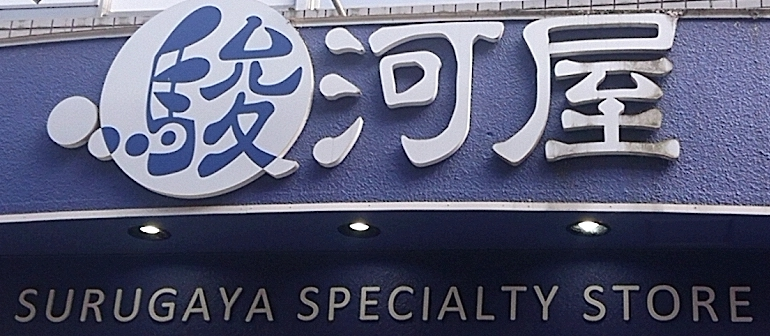
\includegraphics[clip, height=2zh]{surugaya.jpg}
        \end{minipage} & 10 & 10 \\
        \hline
      \end{tabular}
    \end{center}
  \end{table}
